\documentclass[a4paper,12pt]{article}
\usepackage[authoryear]{natbib}
\usepackage{jabes}
\usepackage{mathtools}
\usepackage{wrapfig}
\usepackage{fancyvrb}

%% Language %%%%%%%%%%%%%% %%%%%%%%%%%%%%%%%%%%%%%%%%%%%%%%%%%
\usepackage[french]{babel} 
\usepackage[T1]{fontenc}
\usepackage[utf8]{inputenc}
\usepackage{caption}
\usepackage{color}
\def\r#1{\textcolor{blue}{\bf[#1]}}
\newcounter{interrogation}
\def\q#1{\refstepcounter{interrogation}\textcolor{red}{\bf[Q\arabic{interrogation}. #1]}}
\usepackage{hyperref}

\def\vect#1{\bm{#1}}
\def\matx#1{\mathbf{#1}}

\newcommand{\citetapos}[1]{\citeauthor{#1}'s \citeyearpar{#1}}

\newcommand{\authorlist}{Fortin, M.}
\newcommand{\runninghead}{MATHILDE}
\title{Le simulateur MATHILDE \\ dans CAPSIS}
\author{Mathieu Fortin et Rubén Manso}
\date{\today}

\begin{document}
\maketitle
\tableofcontents

\listoffigures
\listoftables

\newpage

\section{Présentation du simulateur MATHILDE}

\subsection{Introduction}

MATHILDE est un simulateur de croissance conçu pour les hêtraies-chênaies du Nord de la France. Ces composantes principales ont été ajustées à partir des données du réseau de placettes permanentes du Laboratoire d'Etude des Ressources Forêt-Bois (LERFoB). Plus précisément, ce sont les données de 72 placettes mesurées entre 1958 et 2007 qui ont été mises à contribution. La distribution géographique de ces placettes est illustrée dans la Figure~\ref{figureDistributionPlacettes}.

\begin{figure}[h]
	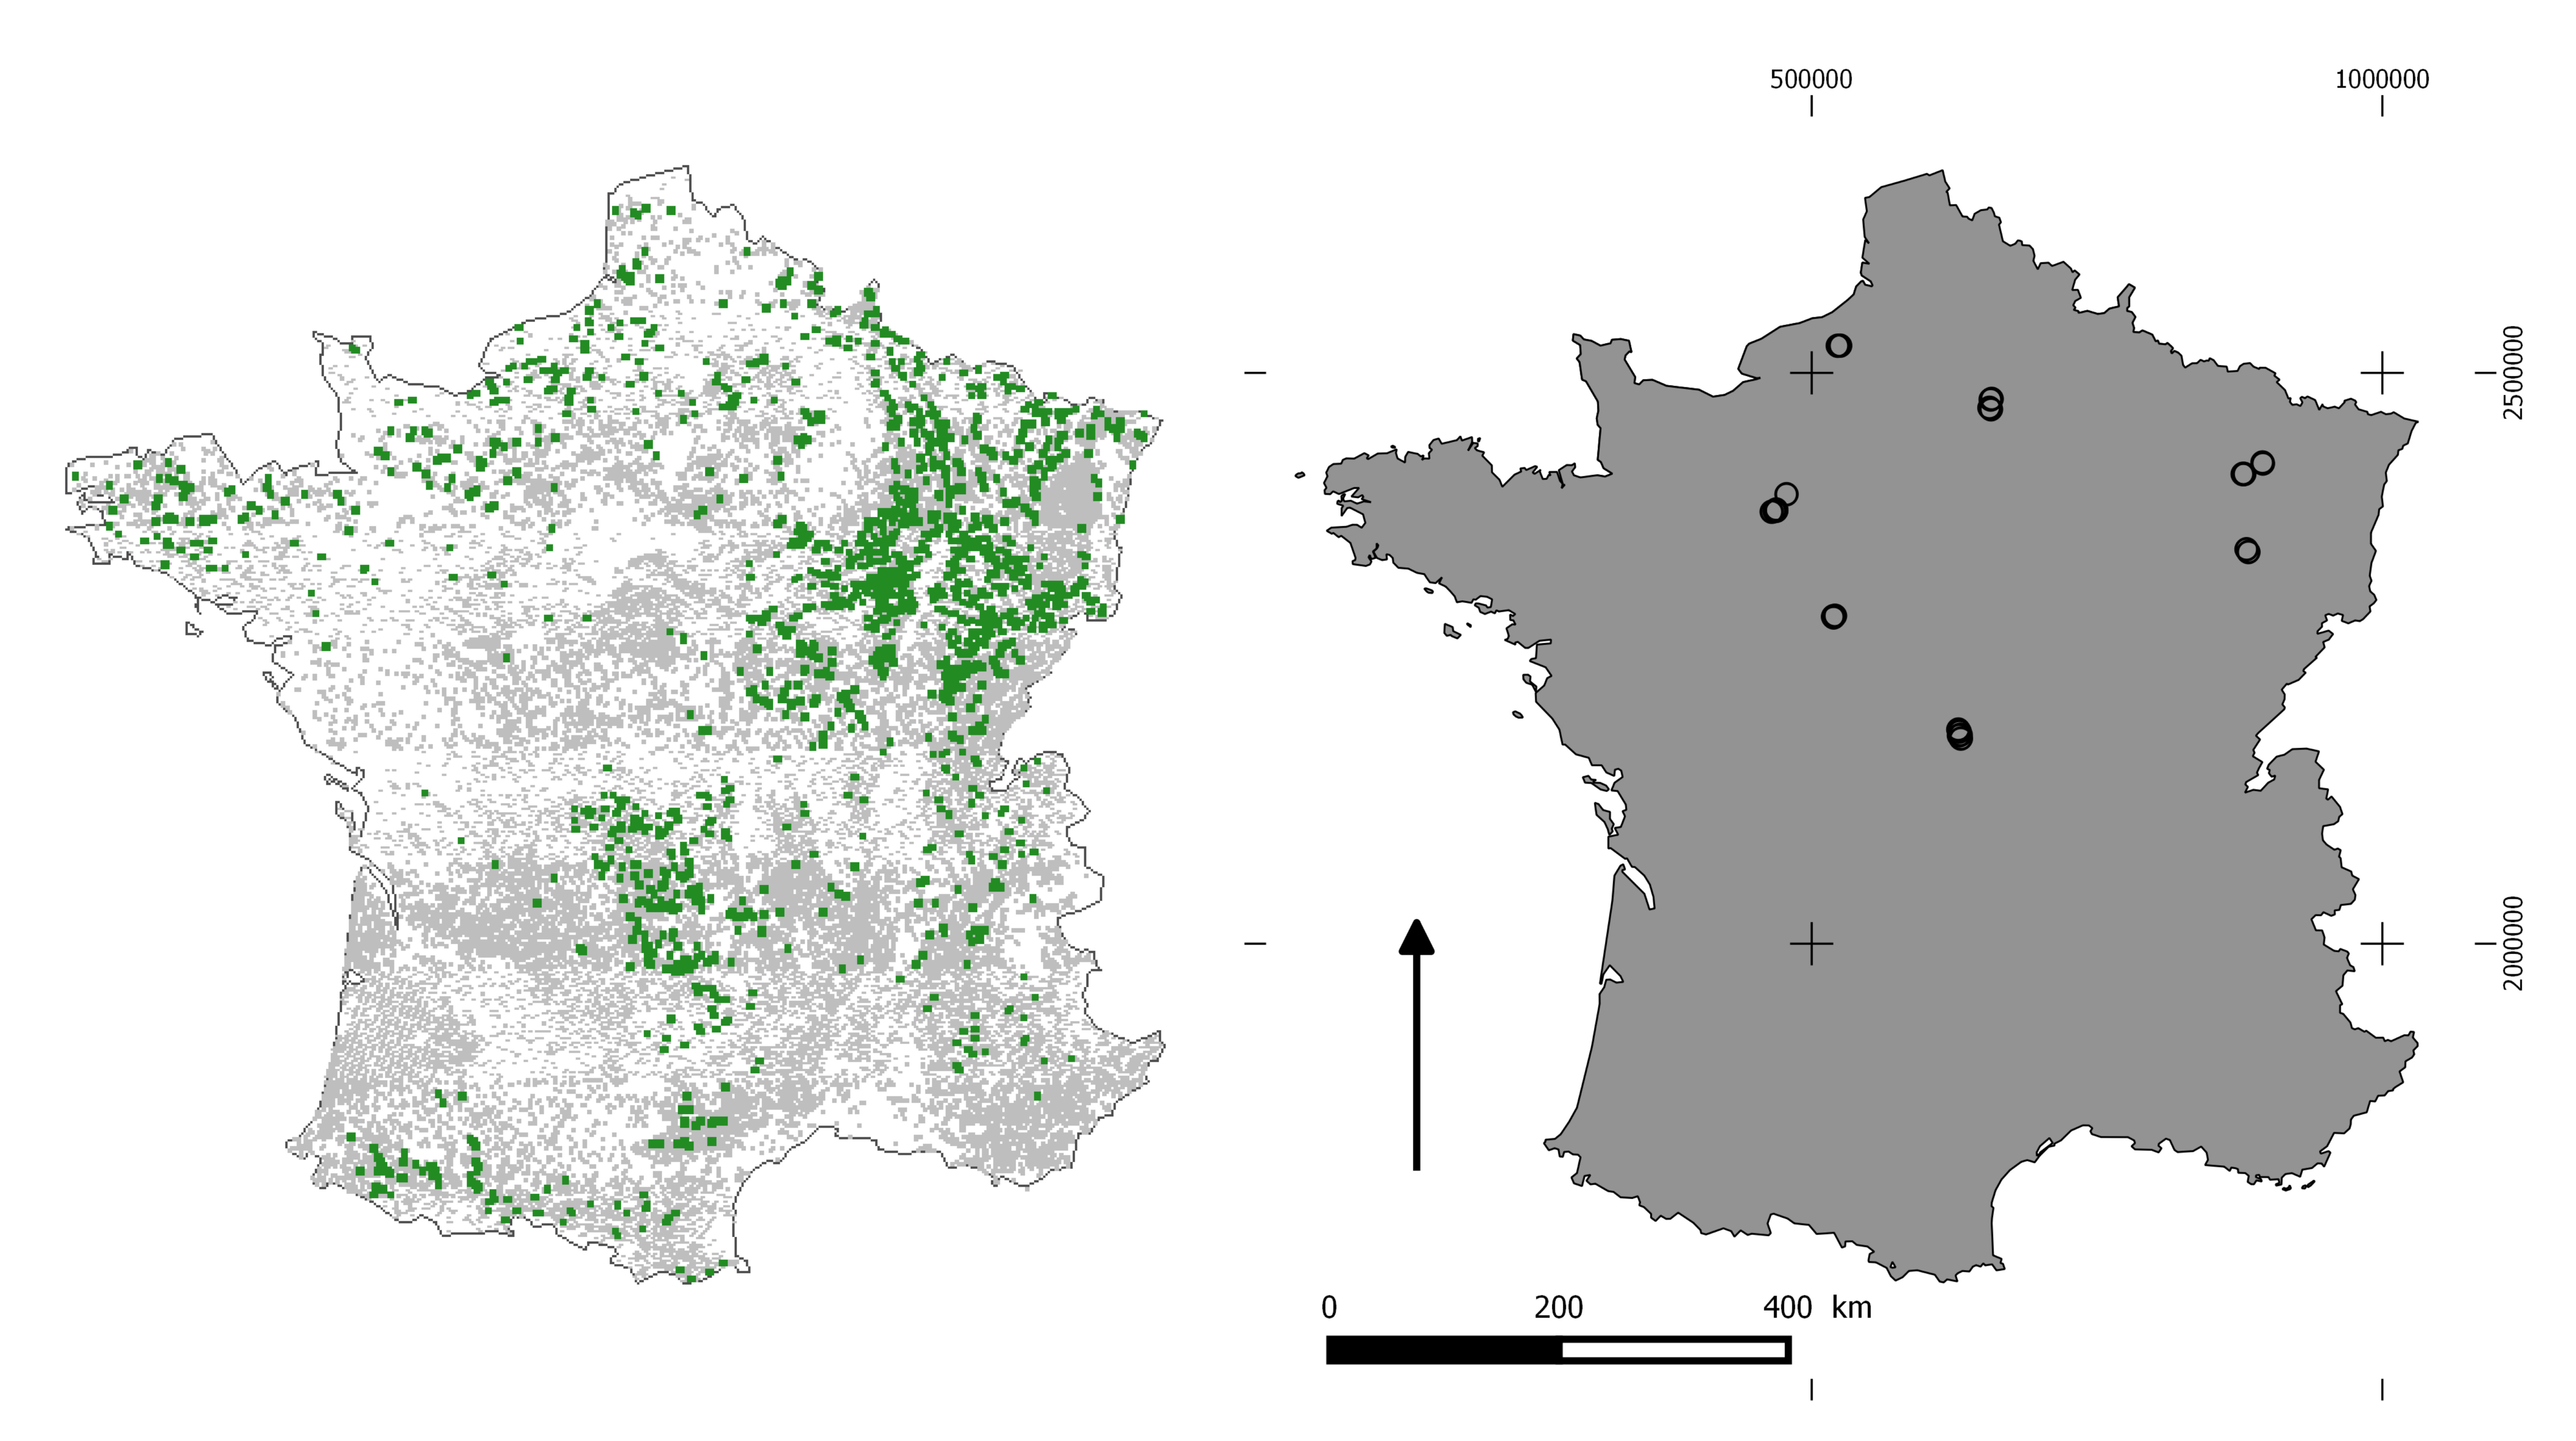
\includegraphics[width=\textwidth]{./figures/distributionPlacettes}
	\caption{Distribution des placettes l'inventaire forestier national contenant du chêne et du hêtre (à gauche) et des placettes du réseau LERFoB (à droite).}
	\label{figureDistributionPlacettes}
\end{figure}

Ce simulateur a été conçu en collaboration avec le département Recherche, Développement et Innovation (RDI) de l'Office National des Forêts (ONF) dans le but, non pas de remplacer le simulateur FAGACEES \citep[cf.][]{dhote_beech_1996}, mais plutôt d'apporter une vision complémentaire du fait d'une approche de modélisation différente. En effet, sa construction basée sur une approche par tiges individuelles offre une plus grande flexibilité. Son usage n'est pas restreint aux peuplements réguliers de chêne ou de hêtre comme FAGACEES. MATHILDE permet de prévoir la croissance du mélange de ces deux espèces.

\subsection{Données d'ajustement}

Les placettes du réseau LERFoB ont des surfaces qui varient entre 0,2 et 2,0~ha. Elles ont été remesurées à des intervalles qui varient entre 1 et 10 ans. Compte tenu du nombre d'espèces (\hyperref[Annexe1]{Annexe 1}), nous avons procédé au regroupement suivant:

\begin{itemize}
  \item Hêtre
  \item Chênes (sessiles en grande majorité et pédonculés)
  \item Charme
  \item Autres espèces
\end{itemize}

La base de données comptait plusieurs dizaines de milliers d'observations d'arbres (Tableau~\ref{tableSommaireData}). Dans près de la moitié des placettes, on pouvait observer un mélange de chêne et de hêtre dans des proportions très variables. La Figure~\ref{figGvsN} montre la distribution des surfaces terrières en fonction de la densité de tiges.

\begin{table}[h]
\begin{center}
\caption{Sommaire du jeu de données}
\label{tableSommaireData}
\begin{tabular}{lcccc}
\hline
	& Hêtre & Chênes & Charme & Autres \\
\hline
Nombre d'observations & 65~314 & 111~083 & 3899 & 106 \\
Nombre d'arbres morts & 1424 & 1276 & 157 & 6 \\
$\text{d}_{130}$ (cm) & 4,5 -- 108,5 & 6,1 -- 142,6 & 5,4 -- 39,2 & 7,0 -- 38,2 \\
Surface terrière (m$^2$ha$^{-1}$) & 5,8 -- 64,3 & 4,5 -- 59,4 & 11,2 -- 56,4 & 11,6 -- 49,0 \\
Densité (tiges ha$^{-1}$) & 28 -- 2620 & 34 -- 2620 & 94 -- 2155 & 172 -- 2135 \\
Durée de l'intervalle (années) & 1 -- 10 & 1 -- 10 & 1 -- 10 & 1 -- 10 \\ 
\hline
\end{tabular}
\end{center}
\end{table}

\begin{figure}[h]
\begin{center}
	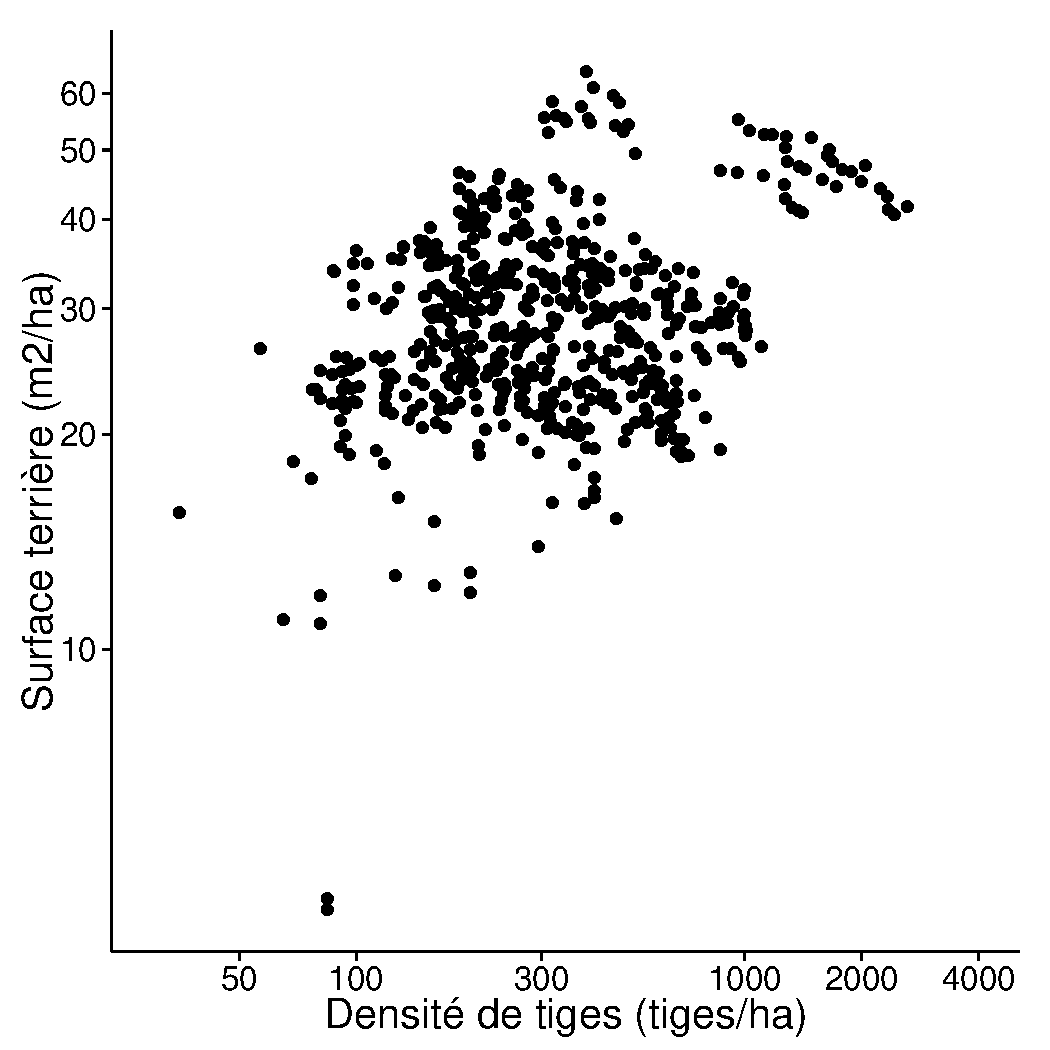
\includegraphics[width=0.5\textwidth]{./figures/lerfobGagainstN_fr}
	\caption{Surface terrière en fonction de la densité de tiges dans le jeu de données d'ajustement.}
	\label{figGvsN}
\end{center}
\end{figure}

\subsection{Fonctionnement}

Ce simulateur de croissance est un modèle par arbres individuels indépendant des distances. Il fonctionne à partir des données dendrométriques de base comme la hauteur et le diamètre et comprend 6 modules (Figure~\ref{figureOrganigramme}):

\begin{itemize}
  \item Module de mortalité
  \item Module d'accroissement en diamètre à 1,3 m de hauteur ($\text{d}_{130}$)
  \item Module d'estimation de la hauteur des arbres
  \item Module d'estimation du volume bois fort tige
  \item Module d'estimation de la probabilité de récolte
  \item Module de température
\end{itemize}

Les modules de mortalité et d'accroissement en diamètre permettent de prévoir les changements sur un intervalle de croissance de 1 à 10 ans, 5 ans étant la durée suggérée lors de l'utilisation dans CAPSIS. Les modules de hauteur et de volume permettent d'estimer ces variables à partir de caractéristiques données à un moment précis. Le module de probabilité de récolte définit la probabilité qu'une placette subisse une intervention et le cas échéant, la probabilité de récolte propre à chaque arbre de la placette. Le module de température permet de prévoir une température moyenne lors de la saison de croissance dans le prochain intervalle, laquelle influence l'accroissement en diamètre des tiges.

\begin{figure}[h]
\begin{center}
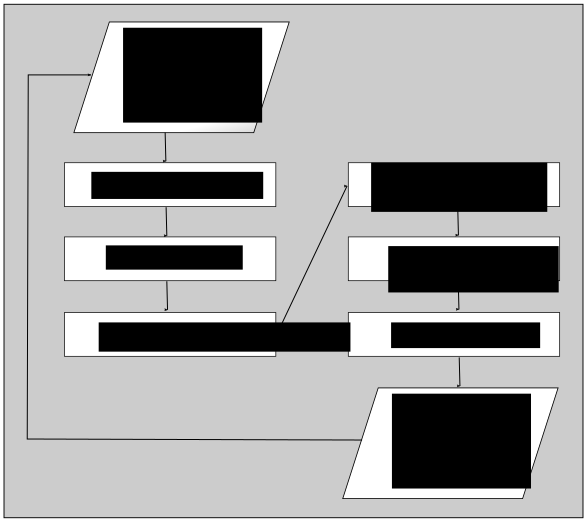
\includegraphics[width=0.6\textwidth]{./figures/flowchart_fr}
\caption{Organigramme du fonctionnement de MATHILDE au cours d'un intervalle de croissance de 5 ans.}
\label{figureOrganigramme}
\end{center}
\end{figure}

Pour obtenir des projections de croissance sur des intervalles plus longs, le simulateur utilise un procédé itératif (Figure~\ref{figureSimulIter}). Par exemple, les prévisions obtenues pour un intervalle de 5 ans sont réinsérées dans le simulateur pour obtenir une prévision sur 10 ans et ainsi de suite jusqu'à ce que l'on atteigne la durée de projection désirée.

\begin{figure}[h]
\begin{center}
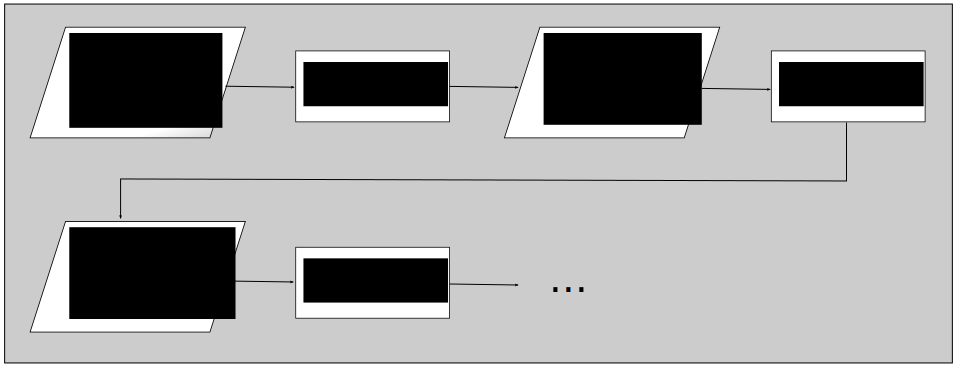
\includegraphics[width=\textwidth]{./figures/simulIter_fr}
\caption{Fonctionnement itératif de MATHILDE afin d'obtenir des prévisions sur des horizons de plus de 5 ans.}
\label{figureSimulIter}
\end{center}
\end{figure}

Le simulateur peut fonctionner sous deux modes: le mode déterministe et le mode stochastique. En mode déterministe, tous les modules fournissent une estimation de l'espérance. En mode stochastique, on commence par recopier la liste d'arbres initiale un certain nombre de fois. Ensuite, on simule l'évolution de chacune des copies en tirant aléatoirement des valeurs dans les lois de distribution auxquelles appartiennent divers éléments du simulateur. MATHILDE utilise une approche complètement stochastique: on tente de simuler l'ensemble de la variabilité du simulateur. Ainsi des valeurs sont tirées afin de représenter 

\begin{itemize}
	\item les erreurs associées aux estimations des paramètres des modules
	\item les effets aléatoires de placette, d'intervalle et d'arbre lorsqu'il y en a
	\item les erreurs résiduelles
\end{itemize}

Puisqu'il est très peu probable que les m\^emes valeurs soient tirées pour deux copies de la liste d'arbres initiale, chacune d'elles aura donc une évolution distincte. Ces évolutions de croissance associées à chaque copie sont appelées réalisations (Figure~\ref{figureMCApproach}). Plus le nombre de réalisations est grand, plus on reproduit la variabilité naturelle liée à la croissance.

En dépit des temps de calcul plus longs, le mode stochastique est très utile pour obtenir un intervalle de confiance autour des prévisions, ce qui est impossible en mode déterministe. Par ailleurs, le mode déterministe induit vraisemblablement un léger biais dans les prévisions à moyen et long termes en raison de la non-linéarité des modules qui composent le simulateur \citep{fortin_stochastic_2012}.

\begin{figure}[h]
\begin{center}
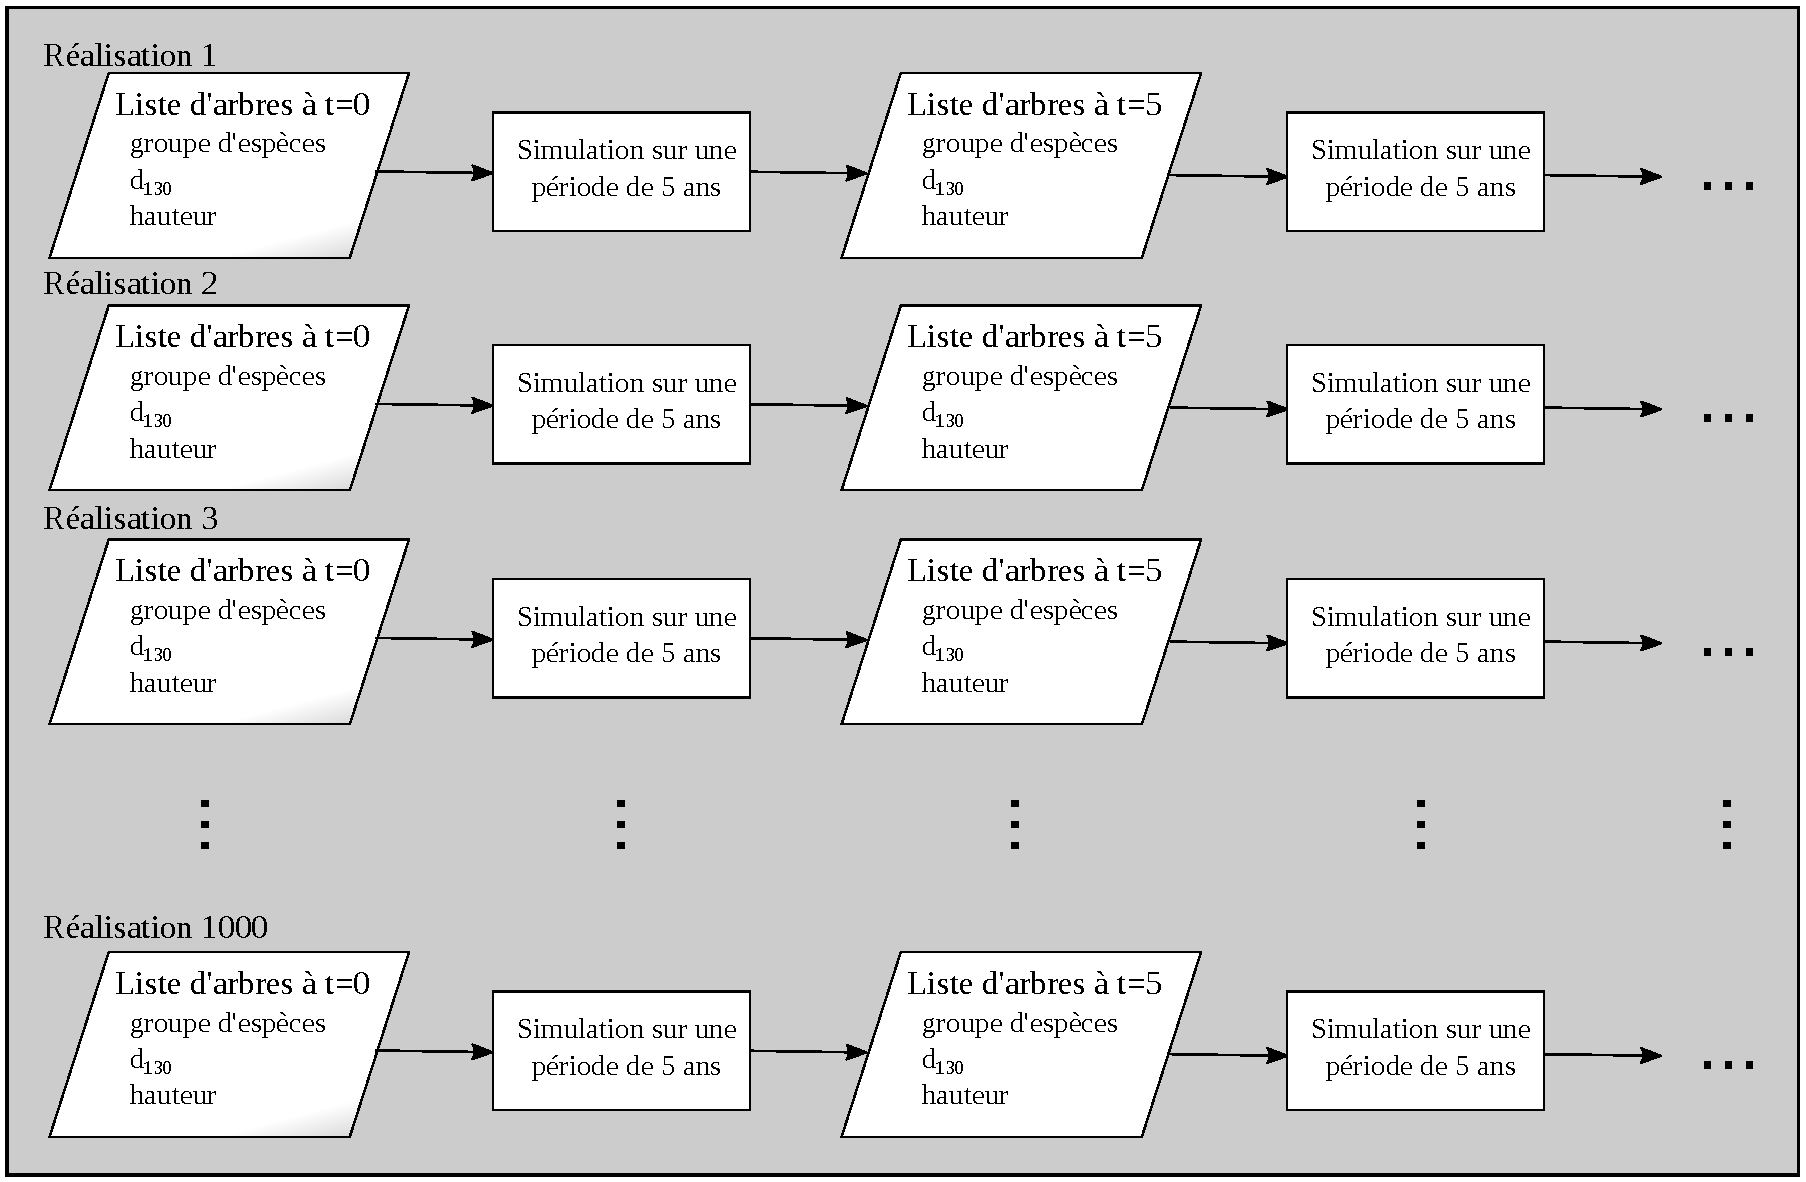
\includegraphics[width=\textwidth]{./figures/mcApproach_fr}
\caption{Exemple d'une simulation stochastique basée sur 1000 réalisations.}
\label{figureMCApproach}
\end{center}
\end{figure}

Les modules de hauteur, de volume, de climat et de température font l'objet de manuscrits qui sont en cours de rédaction. Les prochaines sections portent plut\^ot sur le c\oe{}ur du modèle soit les modules de mortalité et d'accroissement en diamètre.

\subsubsection{Module de mortalité}

Le module de mortalité prévoit une probabilité de mortalité d'un arbre donné sur une période de 1 à 10 ans. Si $m$ est une variable binaire de sorte que si l'arbre meurt $m=1$ et s'il survit $m=0$, alors le module de mortalité peut s'exprimer sous la forme suivante:

\begin{equation}
\text{Pr}(m=1) = 1 - e^{-e^{\vect{x}\vect{\beta}}}
\end{equation}

où $\vect{x}$ est un vecteur de variable explicative et $\vect{\beta}$ est un vecteur de paramètres. Les variables explicatives contenues dans $\vect{x}$ sont les suivantes:

\begin{itemize}
  \item le groupe d'espèces
  \item le d130
  \item la surface terrière en hêtre des arbres dont le d130 est plus élevé que le sujet
  \item la surface terrière en chêne des arbres dont le d130 est plus élevé que le sujet
  \item l'occurence d'une tempête
  \item l'occurence d'une sécheresse
  \item l'occurence d'une coupe
  \item la durée de l'intervalle
\end{itemize}

Un effet aléatoire d'intervalle a été ajouté en interaction à l'occurrence de tempête afin de mieux recréer l'hétérogénité des dommages de tempête dans les peuplements. Les détails de ce module sont disponibles dans \citet{manso_mortalite_2015}. 

\subsubsection{Module d'accroissement en diamètre}

Le module d'accroissement en diamètre prévoit l'accroissement d'un arbre donné sur un intervalle de 2 à 10 ans, 5 ans étant la durée recommandée lorsqu'on utilise MATHILDE. Si $i$, $j$ et $k$ sont les indices des placettes, des arbres et des intervalles, alors le module s'exprime de la façon suivante:

\begin{equation}
ln(\Delta \text{d}_{130,ijk} + 1)  = \vect{x} \vect{\beta} + u_i + u_{ij} + \epsilon_{ijk}
\end{equation}

où $\Delta \text{d}_{130,ijk}$ est l'accroissement en diamètre de l'arbre $j$ dans la placette $i$ au cours de l'intervalle $k$, $\vect{x}$ est un vecteur de variable explicative, $\vect{\beta}$ est un vecteur de paramètres, $u_i$ et $u_{ij}$ sont des effets aléatoires de placette et d'arbre, lesquels suivent des lois normales, et $\epsilon_{ijk}$ est le terme d'erreur résiduelle.

Les variables explicatives qui ont un effet sur l'accroissement en diamètre sont:

\begin{itemize}
  \item le groupe d'espèces
  \item le d130
  \item la surface terrière en hêtre des arbres dont le d130 est plus élevé que le sujet
  \item la surface terrière en chêne des arbres dont le d130 est plus élevé que le sujet
  \item la surface terrière de la placette
  \item l'occurence d'une coupe
  \item la durée de l'intervalle
  \item la température moyenne de la saison de croissance au cours de l'intervalle
\end{itemize}

Les détails de ce module sont disponibles dans \citet{manso_accr_2015}. 

\subsection{Avantages et limites d'utilisation}

Par rapport à FAGACEES, le simulateur MATHILDE présente certains avantages, notamment les suivants:

\begin{itemize}
  \item il permet de prévoir l'évolution des mélanges;
  \item il fournit un intervalle de confiance associé aux prévisions;
  \item il considère l'impact des tempêtes et des sécheresses; 
  \item il inclut une variable climatique.
\end{itemize}

Comme les gestionnaires forestiers sont généralement intéressés par la croissance des strates d'inventaire ou des peuplements, le simulateur permet aussi de simuler plusieurs placettes dans un même fichier d'inventaire. Ainsi, il est possible de simuler une strate de quinze placettes en mettant ces placettes bout à bout dans le fichier d'inventaire. MATHILDE simule la croissance de chacune d'elles séparément et affiche la moyenne des quinze évolutions.

Le simulateur MATHILDE actualise des placettes dans le temps. Les placettes qu'il utilise sont des placettes à surface fixe. En raison des biais liés à la surface de placette \citep[cf.][]{sambakhe_bias_2014}, \textbf{on recommande d'utiliser des placettes dont la surface se situe entre 400 m$^2$ et 1 ha}. 

Le simulateur est conçu pour simuler la croissance de peuplements gérés. \textbf{En l'absence d'éclaircies, il aura tendance à surestimer la croissance}. Comme il n'y a pas de recrutement, le simulateur ne peut reproduire un passage à la futaie jardinée. \textbf{Il tendra donc à sous-estimer l'accroissement sur les horizons assez longs en raison de l'absence de recrutement.}

Les données ayant servi à l'ajustement des modules de mortalité et d'accroissement en diamètre ne comportent que très peu de tiges de moins de 5 cm de diamètre. \textbf{La simulation de peuplements juvéniles (en deça de 30 ans d'âge) est susceptible de donner des résultats aberrants, particulière pour le chêne où les probabilités de mortalité sont fortement surestimées}. 

Les peuplements gérés sont habituellement récoltés lorsqu'ils atteignent un diamètre dominant de 65 cm. \textbf{Si on poursuit la simulation au-delà de ce seuil, les probabilités de mortalité pour les arbres de fortes dimensions ($\text{d}_{130}$ > 65 cm) tendent à être sous-estimées, ce qui entraîne inévitablement une surestimation de la croissance.}

\subsection{Evaluation du simulateur}

Chacun des modules du simulateur a été évalué par validation croisée. Une fois que ces évaluations se sont avérées satisfaisantes, ils ont été assemblés pour former MATHILDE (Figure~\ref{figureOrganigramme}). Le comportement global du simulateur a aussi été évalué par validation croisée. Des statistiques comme les biais et les racines des erreurs quadratiques moyennes des prévisions en surface terrière et en nombre de tiges à l'hectare ont été calculées (Tableau~\ref{TableEvaluationLERFoB}). Les valeurs observées ont également été comparées aux valeurs prédites (Figure~\ref{figureComparObsPred}).

\begin{table}[!h]
\begin{center}
\caption{Evaluation de MATHILDE par validation croisée ($n$: nombre d'intervalles de croissance, REQM: racine de l'erreur quadratique moyenne, les valeurs relatives sont entre parenthèses).}
\label{TableEvaluationLERFoB}
\begin{tabular}{llccc}
\hline
Variable & Contexte & $n$ & Biais & REQM \\
\hline
Densité de tiges (tiges ha$^{-1}$) & Sans coupe & 204 & 9,1 (2,2\%) & 48.7 (11,7\%) \\
				& Avec coupe & 175 & 11,7 (3,9\%) & 40,0 (13,5\%) \\
Surface terrière (m$^2$ha$^{-1}$) & Sans coupe & 204 & 0,2 (0,7\%) & 6,8 (20,9\%) \\
 				& Avec coupe & 175 & 1,5 (5,3\%) & 4,5 (16,1\%) \\
 \hline
\end{tabular}
\end{center}
\end{table}

\begin{figure}[!h]
\begin{center}
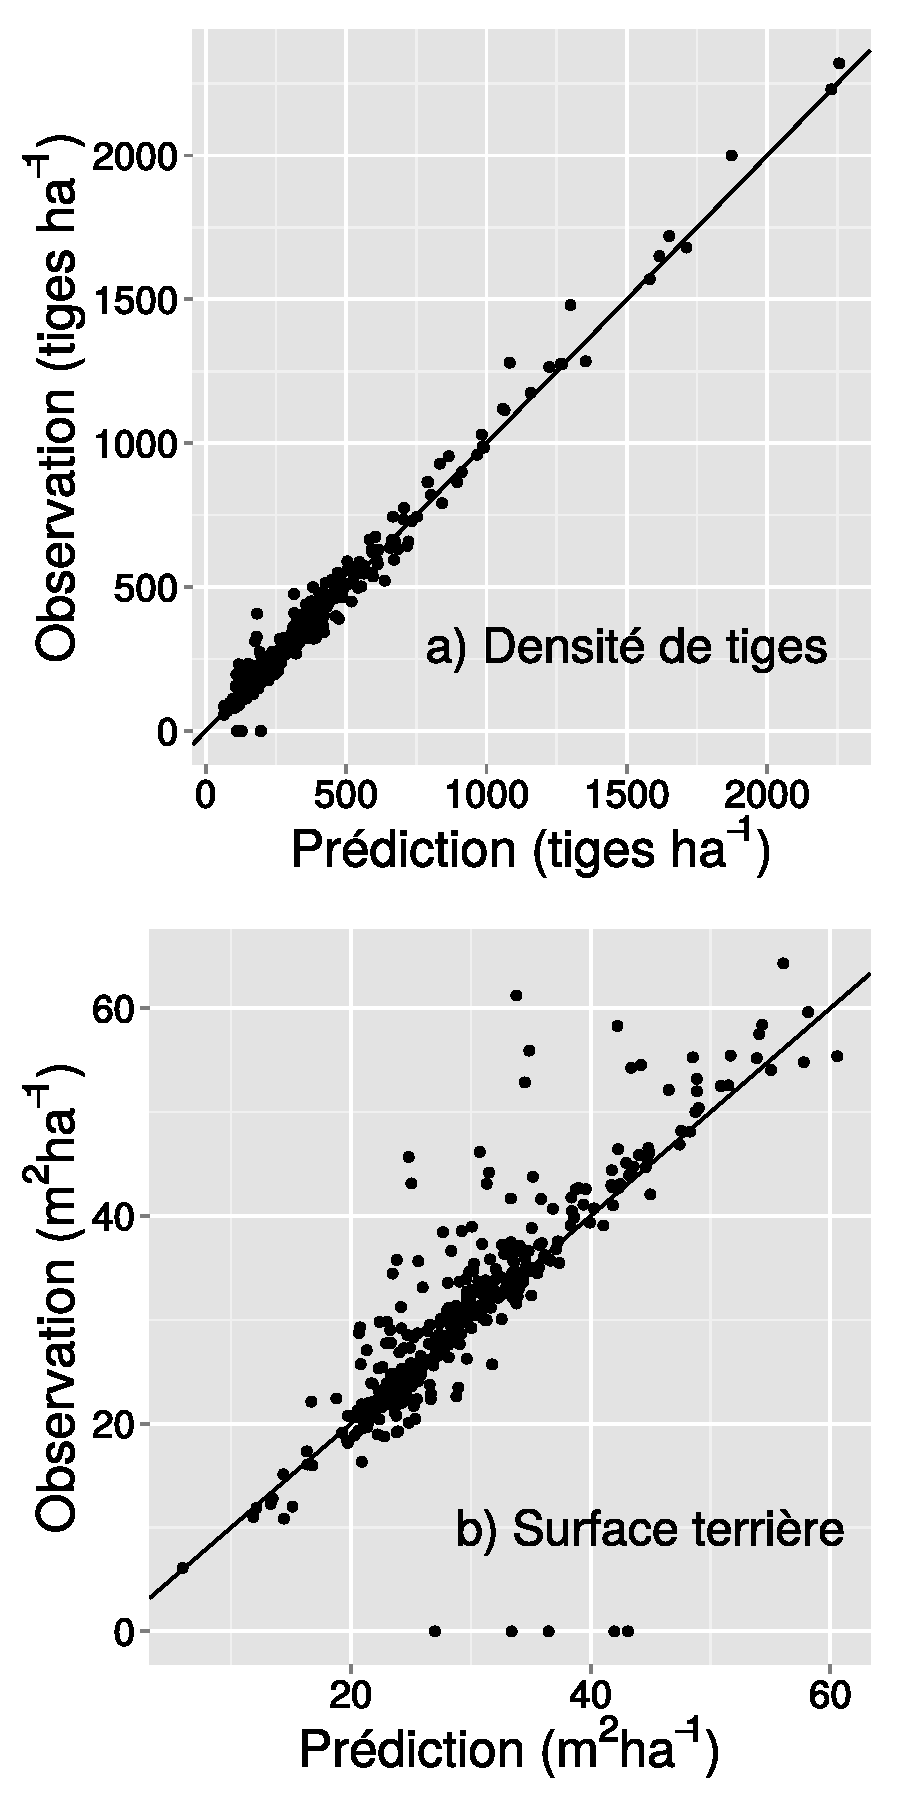
\includegraphics[width=7cm]{./figures/stochasticEvaluationGraphfr}
\caption{Comparaison entre les valeurs observées et prédites par MATHILDE.}
\label{figureComparObsPred}
\end{center}
\end{figure}


\subsection{Contributions}

Les auteurs de ce document tiennent à remercier François Morneau (ONF-IGN), François Ningre (LERFoB), Christine Deleuze (ONF), Quentin Girard (ONF), Didier François (ONF) et Philippe Dreyfus (ONF) pour leurs suggestions lors des ajustements des modules de mortalité et d'accroissement en diamètre de MATHILDE et de l'évaluation du simulateur. 

\section{Initialiser une simulation}

Le menu d'initialisation de MATHILDE est présenté à la Figure~\ref{figureInitialMenu}. Ce menu vous permet de lire votre fichier d'inventaire et de spécifier l'année de départ de votre simulation.

\begin{figure}[h]
\begin{center}
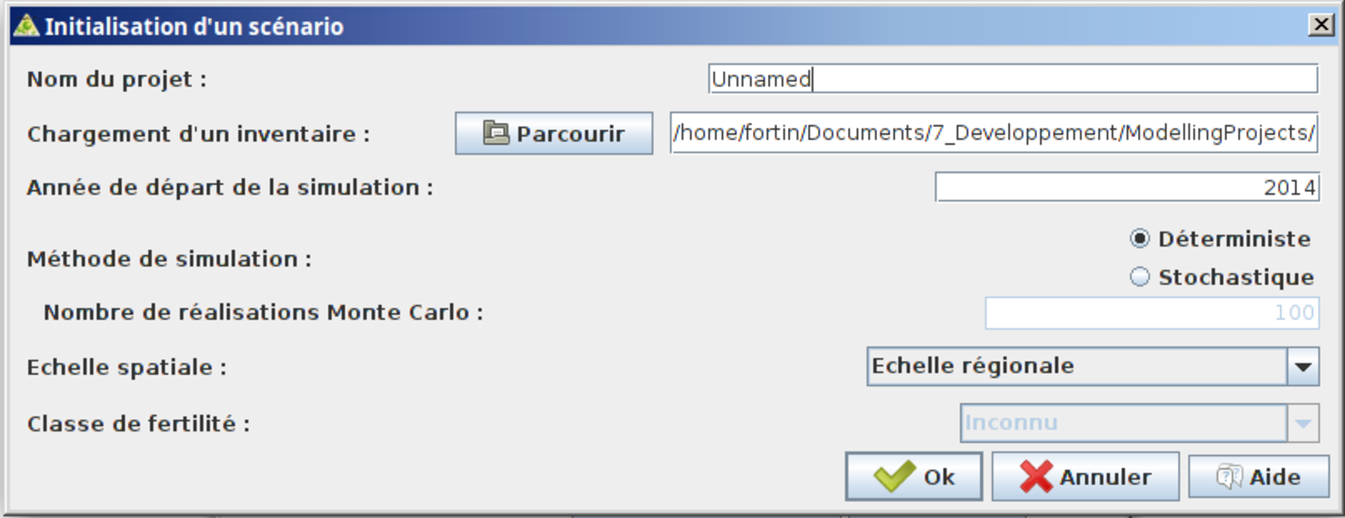
\includegraphics[width=\textwidth]{./figures/initialMenu_fr}
\caption{Menu d'initialisation d'une simulation de MATHILDE.}
\label{figureInitialMenu}
\end{center}
\end{figure}


\subsection{Nom du projet}

Vous pouvez entrer un nom qui caractérise votre projet. 

\subsection{Chargement d'un inventaire}
Vous devez saisir le nom d'un fichier contenant les données d'inventaires. Les fichiers éligibles sont des fichiers de format dBase IV (.dbf) ou texte (.csv). Chaque ligne d'un fichier d'inventaire représente un arbre ou un groupe d'arbres pourvus des mêmes caractéristiques. Chaque ligne doit comprendre les variables suivantes:

\begin{enumerate}
  	\item Identifiant de la strate (facultatif)
    \begin{itemize}
     	\item Si votre fichier d'inventaire comprend plusieurs strates ou plusieurs peuplements, le fait d'identifier ce champ vous permettra de sélectionner une des strates ou un des peuplements. Si aucun nom de champ n'est fourni, l'importateur considère que le fichier ne comprend qu'une seule strate ou peuplement.
    \end{itemize} 
  	\item Identifiant de placette
    \begin{itemize}
		\item Il s'agit de l'identifiant de vos placettes dans votre fichier (p.ex.: 1, 2, 3, ...).
    \end{itemize} 
    \item Département
    \begin{itemize}
    		\item Le code du département dans lequel se trouve la placette (p.ex. 54, 88). Ce code permettra d'attribuer des coordonnées géographiques à vos placettes dans le cas où celles-ci ne seraient pas disponibles. 
    \end{itemize}
    \item Latitude (facultatif)
    \begin{itemize}
    		\item La latitude de la placette (p.ex. 49.543). Cette variable permet de mieux prévoir la température moyenne de la saison de croissance qui entre dans le module d'accroissement en diamètre.
    \end{itemize}
    \item Longitude (facultatif)
    \begin{itemize}
    		\item La longitude de la placette (p.ex. 2.008). Cette variable permet de mieux prévoir la température moyenne de la saison de croissance qui entre dans le module d'accroissement en diamètre.
    \end{itemize}
  	\item Surface de placette (ha)
    \begin{itemize}
	     \item Il s'agit de la superficie de la placette dans laquelle se trouve ces arbres. ATTENTION: MATHILDE gère les placettes de surfaces différentes au sein d'un inventaire, mais pas les placettes concentriques en un même point d'échantillonnage.
    \end{itemize}   
    \item Code d'essence de l'arbre (CHS, HET, CHA ou autres, voir \hyperref[Annexe1]{Annexe 1})
	\item Diamètre à 1,3 m (cm)
  	\item Fréquence de l'arbre (double exprimé à l'échelle de la placette) (facultatif)
    \begin{itemize}
	\item Il s'agit du nombre d'arbres partageant ces caractéristiques dans la placette. 
    \end{itemize} 
	\item Hauteur de l'arbre (m) (facultatif)
    \begin{itemize}
	\item Si vous disposez de hauteurs mesurées, MATHILDE peut alors les utiliser pour en déduire un effet aléatoire de placette. Si les arbres sont plus grands que la moyenne, ils ont alors tendance à conserver cet avantage dans le temps.
	\end{itemize}     
\end{enumerate}
  
MATHILDE possède un utilitaire d'importation des fichiers de données .dbf ou .csv, lequel vous permettra de préciser les champs qui contiennent les variables mentionnées. Ces variables n'ont donc pas à respecter l'ordre mentionné plus haut. L'utilitaire s'active automatiquement si l'extension de votre fichier est .dbf ou .csv.

Les fichiers d'inventaire peuvent aussi comprendre plus d'une placette. Il est donc possible de simuler des groupes de placettes représentant des peuplements ou des strates d'inventaire.

\subsection{Année de départ de la simulation}

Il s'agit de l'année de départ de la simulation. Par défaut, l'année courante est utilisée. Vous pouvez également travailler sur la base de l'âge. Par exemple, ce champ pourrait contenir la valeur de 30 pour indiquer que le peuplement a 30 ans. ATTENTION: l'âge n'a aucune influence sur l'évolution puisque les composantes de MATHILDE n'utilisent pas cette variable. L'âge est donc seulement une variable indicative pour l'utilisateur. 

L'année de départ de la simulation a une incidence sur la prévision de la température moyenne de la saison de végétation pour les intervalles de croissance de la simulation. En effet, le module de température de MATHILDE induit une augmentation des températures depuis les années 1950. \textbf{N.B. Si l'année entrée est inférieure à 1950, alors la simulation est réalisée sous l'hypothèse que le climat actuel ne se réchauffe pas.}

\subsection{Méthode de simulation}

Le simulateur permet d'effectuer des simulations déterministes ou stochastiques. Les simulations stochastiques permettent d'avoir une idée de l'incertitude associée aux prévisions du simulateur en effectuant plusieurs fois la simulation et en y intégrant des facteurs aléatoires. Il s'agit du procédé que l'on nomme Monte Carlo et chaque simulation de croissance est communément appelée ``réalisation''. En somme, une réalisation est une simulation de croissance individuelle dans laquelle on tire des nombres aléatoires afin de représenter les éléments stochastiques du simulateur, soit

\begin{itemize}
	\item les erreurs dans les estimations de paramètre
  	\item les erreurs résiduelles de module (accroissement, mortalité, etc...)
  	\item les effets aléatoires de placette, d'arbre ou d'intervalle
\end{itemize}

Pour effectuer une simulation déterministe, c'est-à-dire, une simulation basée sur la moyenne uniquement, sélectionnez l'option ``Déterministe''. Pour une simulation stochastique, sélectionnez l'option ``Stochastique'' puis entrez un entier afin de spécifier le nombre de réalisations que vous souhaitez faire. Le simulateur est conçu pour un nombre de réalisations entre 1 et 1000. \textbf{Les concepteurs du modèle recommandent d'utiliser un minimum de 100 itérations Monte Carlo lors des simulations stochastiques.} Notez que le mode stochastique demande plus de ressources et par conséquent, le temps pour obtenir une prévision peut être plus long.

\subsection{Echelle spatiale}

Il existe deux options dans MATHILDE: vous pouvez simuler un peuplement (option par défaut) ou une entité forestière plus grande. L'une ou l'autre de ces options affectent la façon dont sont gérées les perturbations et le tirage des nombres aléatoires dans les simulations stochastiques. Par exemple, dans une simulation stochastique à l'échelle du peuplement, MATHILDE ne générera qu'un seul effet aléatoire de placette pour l'ensemble des placettes. En d'autres termes, MATHILDE présume que les placettes sont suffisamment proche les unes des autres pour que cet effet placette soit le même. Lors de la réalisation d'une coupe ou la simulation d'une tempête, toutes les placettes seront affectées simultanément. 

A l'inverse, l'utilisation de l'option "Régionale" indiquera à MATHILDE que les placettes sont suffisamment loin les unes des autres pour que les effets aléatoires de placette soient différents. Par ailleurs, la coupe pourra être réalisée dans une placette, mais pas dans les autres si celle-ci a atteint les critères requis. Les perturbations peuvent aussi se produire de façon asynchrone.

\subsection{Classe de fertilité (préliminaire)}

Les classes de fertilité sont gérées indirectement en contraignant l'effet aléatoire de placette dans le module de hauteur de MATHILDE. A la base, cet effet aléatoire suit une loi normale. On tronque cette loi de façon à représenter trois classes de fertilité: 

\begin{itemize}
	\item Classe I (les 16 premiers percentiles de la distribution)
	\item Classe II (les 61 percentiles centraux de la distribution)
	\item Classe III (les 23 derniers percentiles de la distribution)
\end{itemize}

L'utilisation d'une classe de fertilité désactive l'estimation de l'effet aléatoire de placette dans le module de hauteur lorsque le fichier d'inventaire contient des hauteurs d'arbres. Aussi, cette option n'est disponible que si l'échelle spatiale est celle du peuplement.

Cette option est actuellement en développement et les percentiles seront mieux définis dans une version ultérieure de MATHILDE.

\subsection{Exemple d'initialisation d'une simulation}
\label{exempleInitialization}

Dans le sous-répertoire data/mathilde/ de votre répertoire capsis/, vous trouverez le fichier hetre.csv. Vous pouvez donc démarrer une simulation stochastique basée sur 100 réalisations en remplissant le dialogue d'initialisation comme dans la Figure~\ref{figureInitEx1}.

\begin{figure}[!h]
\begin{center}
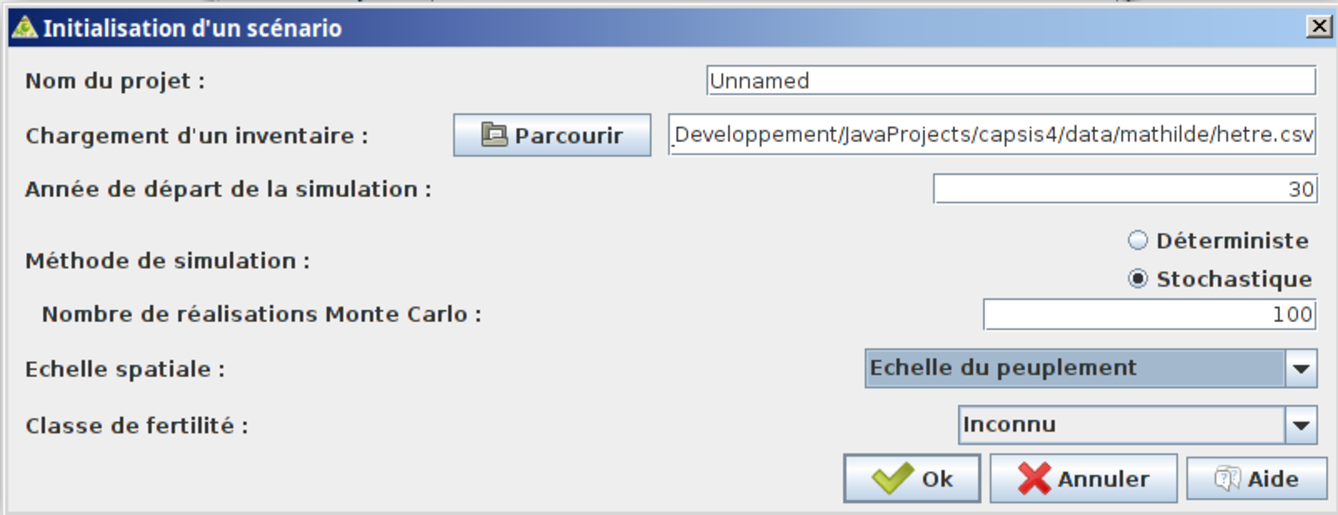
\includegraphics[width=\textwidth]{./figures/initializationExample1}
\caption{Exemple d'initialisation d'une simulation avec un peuplement de hêtre.}
\label{figureInitEx1}
\end{center}
\end{figure}

Lorsque vous cliquez sur Ok, l'utilitaire d'importation de fichier de données apparaîtra. Vous n'avez qu'à faire glisser les champs \textit{d130}, \textit{Espece}, \textit{surfHa}, \textit{placette} et \textit{dep} dans les cases appropriées (Figure~\ref{figureInitEx2}).

\begin{figure}[!h]
\begin{center}
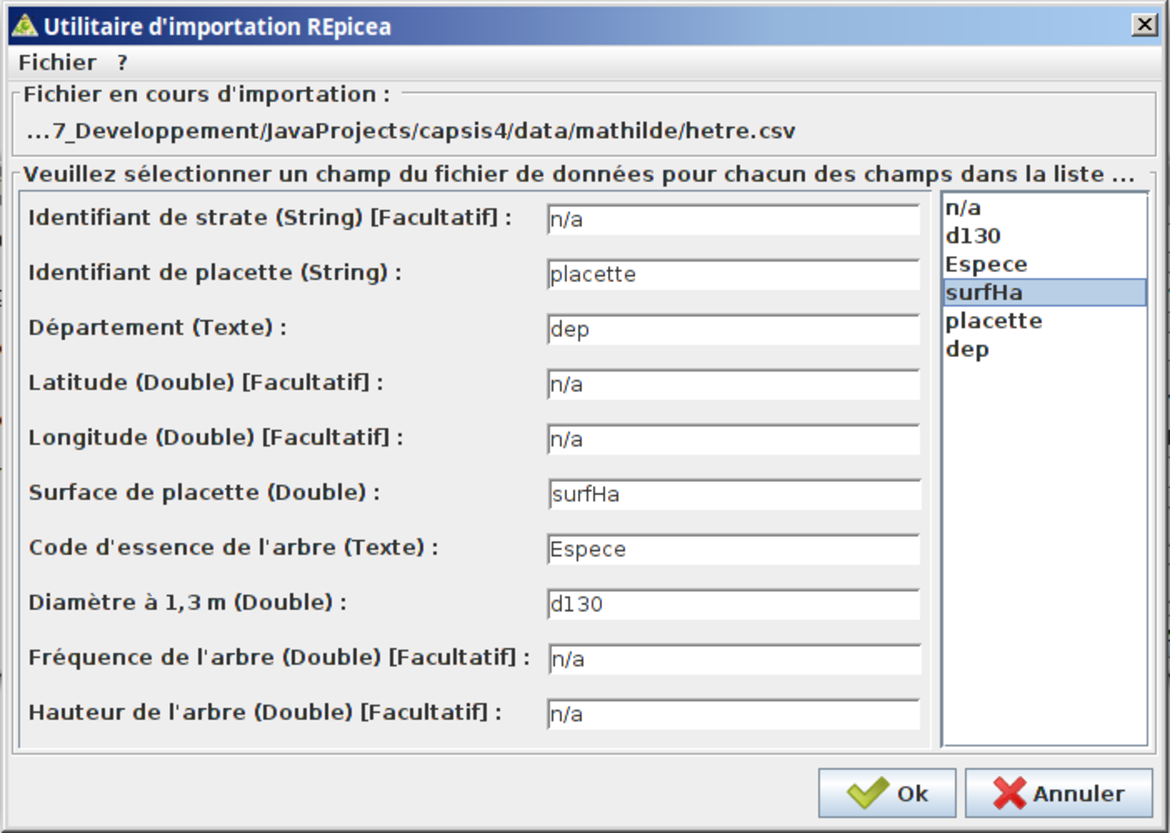
\includegraphics[width=\textwidth]{./figures/initializationExample2}
\caption{Exemple d'utilisation de l'utilitaire d'importation.}
\label{figureInitEx2}
\end{center}
\end{figure}

Lorsque vous cliquez sur Ok, vous obtiendrez un peuplement initial dans la panneau du haut de la fenêtre CAPSIS (Figure\ref{figureInitEx3}).

\begin{figure}[!h]
\begin{center}
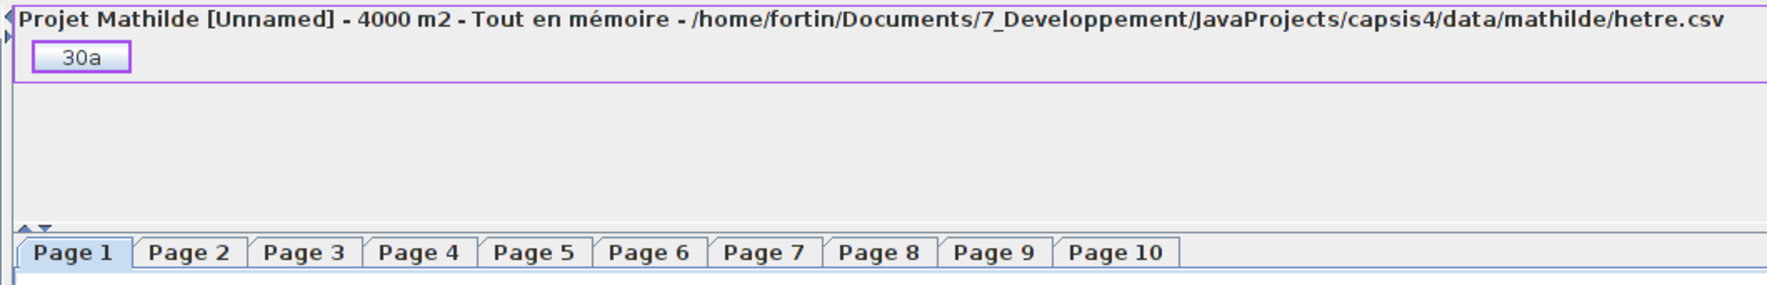
\includegraphics[width=\textwidth]{./figures/initializationExample3}
\caption{Apparition du peuplement initial dans la fen\^etre CAPSIS à la suite de l'importation.}
\label{figureInitEx3}
\end{center}
\end{figure}

\section{Effectuer une évolution}

Vous pouvez faire évoluer une placette ou un groupe de placettes en cliquant bouton droit sur le bouton représentant l'état initial, le bouton marqué ``30a'' dans la Figure~\ref{figureInitEx3}, et en choisissant l'option \textit{Evolution} ou en appuyant sur CTRL+E. Cette action vous menera vers un dialogue d'évolution propre à MATHILDE (Figure~\ref{figureEvolEx1}).

\begin{figure}[!h]
\begin{center}
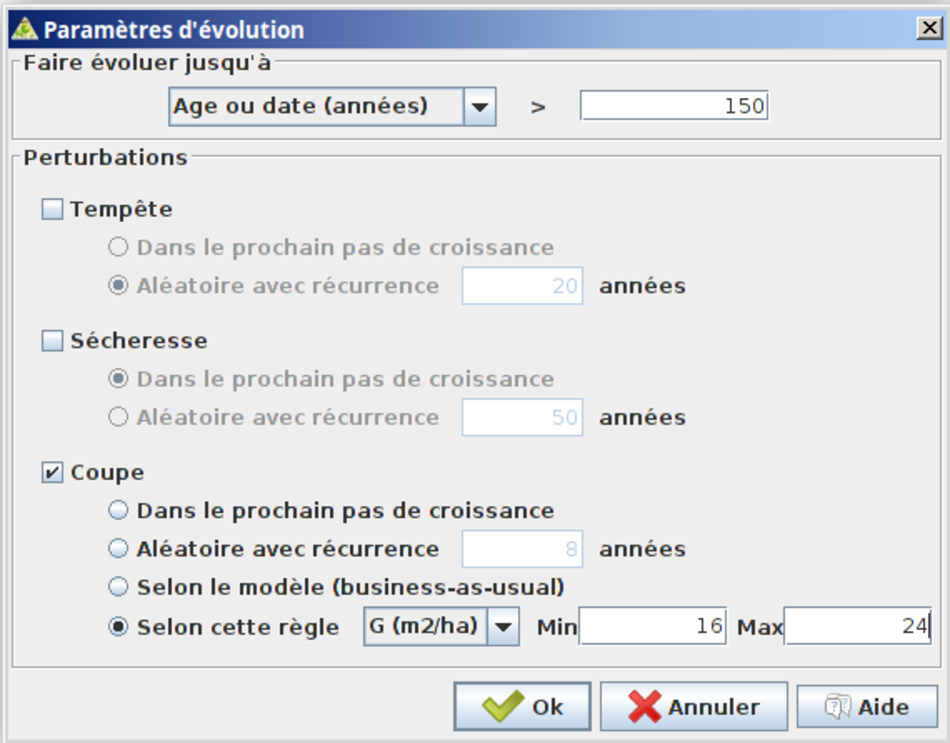
\includegraphics[width=\textwidth]{./figures/evolutionExample1}
\caption{Exemple de paramètres d'évolution dans MATHILDE. L'évolution se fait jusqu'à 150 ans sans temp\^ete ni sécheresse, mais avec une règle de récolte visant à maintenir la surface terrière entre 16 et 24 m$^2$ha$^{-1}$.}
\label{figureEvolEx1}
\end{center}
\end{figure}

\subsection{Faire évoluer jusqu'à}

Il vous est possible de faire évoluer une placette ou un groupe de placettes jusqu'à ce qu'un critère soit atteint. Ce critère peut s'exprimer en 

\begin{itemize}
\item Age ou date (années)
\item Diamètre dominant (cm)
\item Hauteur dominante (m)
\end{itemize}

Le simulateur MATHILDE utilise de préférence des intervalles de 5 ans. Toutefois, si vous choisissez d'utiliser un âge ou une date comme critère d'arrêt, il est possible d'effectuer des simulations sur des horizons qui ne sont pas nécessairement des multiples de 5 ans. Un algorithme redéfinit la longueur des intervalles de façon à effectuer la simulation avec des pas qui se rapprochent de la durée optimale de 5 ans. Par exemple, si votre simulation débute à 30 ans et vous entrez 41 ans, l'algorithme utilisera un intervalle de 6 ans suivi d'un autre de 5 ans. Si vous entrez 38 ans, l'évolution utilise deux intervalles de 4 ans. 

\textbf{Il est fortement recommandé de se limiter à des horizons de simulation ne dépassant pas 60 ans. Au-delà de cet horizon, la précision des prévisions diminue fortement.}

\subsection{Perturbations}

MATHILDE permet de simuler trois types de perturbation: les tempêtes, les sécheresses et les coupes. Dans les trois cas, deux options sont disponibles:

\begin{enumerate}
	\item Dans le prochain pas de croissance
	\begin{itemize}
		\item Le simulateur impose la perturbation dans le premier intervalle de croissance. Supposons que votre simulation débute à 30 ans. Si vous entrez une âge de 55 ans comme critère d'arrêt et vous choisissez d'imposer une tempête dans le prochain pas de croissance, alors la tempête surviendra dans le premier intervalle, soit entre les âges 30 et 35, alors que tous les autres intervalles ne seront pas affectés.
	\end{itemize}
	\item Aléatoire avec récurrence de $x$ années (seulement en mode stochastique)
	\begin{itemize}
		\item Cette option n'est disponible qu'en mode stochastique. Vous pouvez spécifier une récurrence en termes d'années. Si vous entrez 20 ans par exemple, la probabilité annuelle est de 0.05. La probabilité que l'événement survienne au moins une fois au cours d'un intervalle de $t$ ans est alors $1 - (1 - 0.05)^t$.
	\end{itemize}
\end{enumerate}
	
Dans le cas des coupes, deux options additionnelles sont disponibles:

\begin{enumerate}
	\item Selon le modèle (Business as usual) (Seulement en mode stochastique)
	\begin{itemize}
		\item MATHILDE utilise alors son module de coupe pour prévoir la probabilité que la placette soit coupée. Le cas échéant, le simulateur utilise à nouveau le module de coupe pour prévoir la probabilité que chacune des tiges soit récoltée. Il s'agit d'un modèle statistique de récolte décrivant la gestion telle qu'elle a été pratiquée dans les dispositifs du LERFoB au cours des dernières décennies. 
	\end{itemize}
	\item Selon une règle (Seulement à l'échelle du peuplement)
	\begin{itemize}
		\item Cette option n'est disponible que si votre simulation est à l'échelle du peuplement. Vous pouvez définir une règle de récolte sur la base de la surface terrière ou du volume. Vous devez alors définir une borne inférieure et une borne supérieure. Chaque fois que la borne supérieure est franchise, le simulateur enclenche une récolte. Il utilise son module de récolte pour attribuer une probabilité de récolte à chaque arbre. Les arbres sont alors récoltés dans l'ordre décroissant de leur probabilité de récolte jusqu'à ce que la borne inférieure soit atteinte.
	\end{itemize}
\end{enumerate}

\subsection{Exemple d'évolution}

Si nous repartons de l'exemple de la section~\ref{exempleInitialization}, nous pouvons effectuer une évolution jusqu'à 150 ans sans tempête, ni sécheresse mais avec une règle de récolte basée sur la surface terrière (Figure~\ref{figureEvolEx1}). Vous verrez alors apparaître l'évolution dans la fenêtre au haut de l'écran (Figure~\ref{figureEvolEx2}). 

\begin{figure}[!h]
\begin{center}
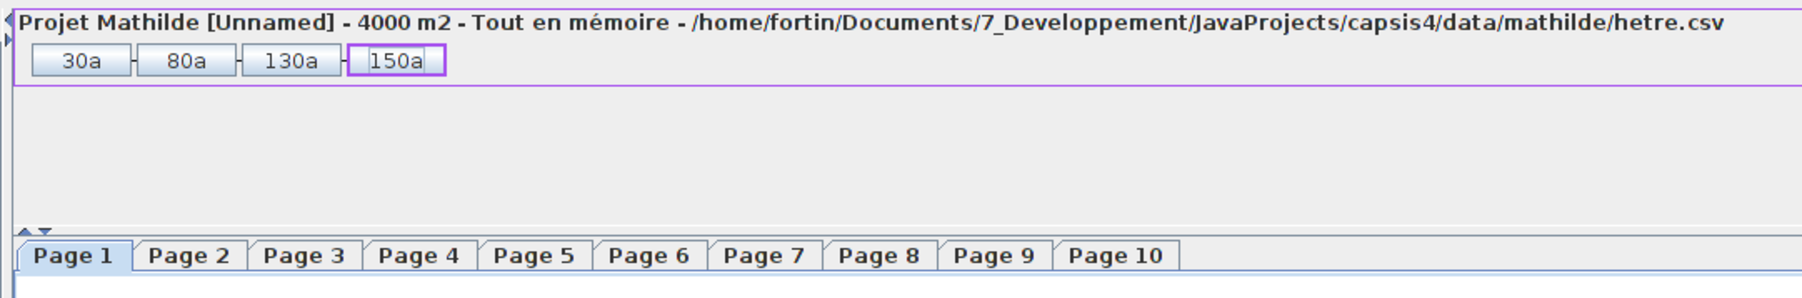
\includegraphics[width=\textwidth]{./figures/evolutionExample2}
\caption{Résultat de l'évolution dans la fen\^etre CAPSIS.}
\label{figureEvolEx2}
\end{center}
\end{figure}

Il est alors possible de visualiser l'évolution en volume en cliquant sur ``IC - Volume'' dans la fenêtre de gauche. Vous verrez apparaître un graphique comme celui de la Figure~\ref{figureEvolEx3}.

\begin{figure}[!h]
\begin{center}
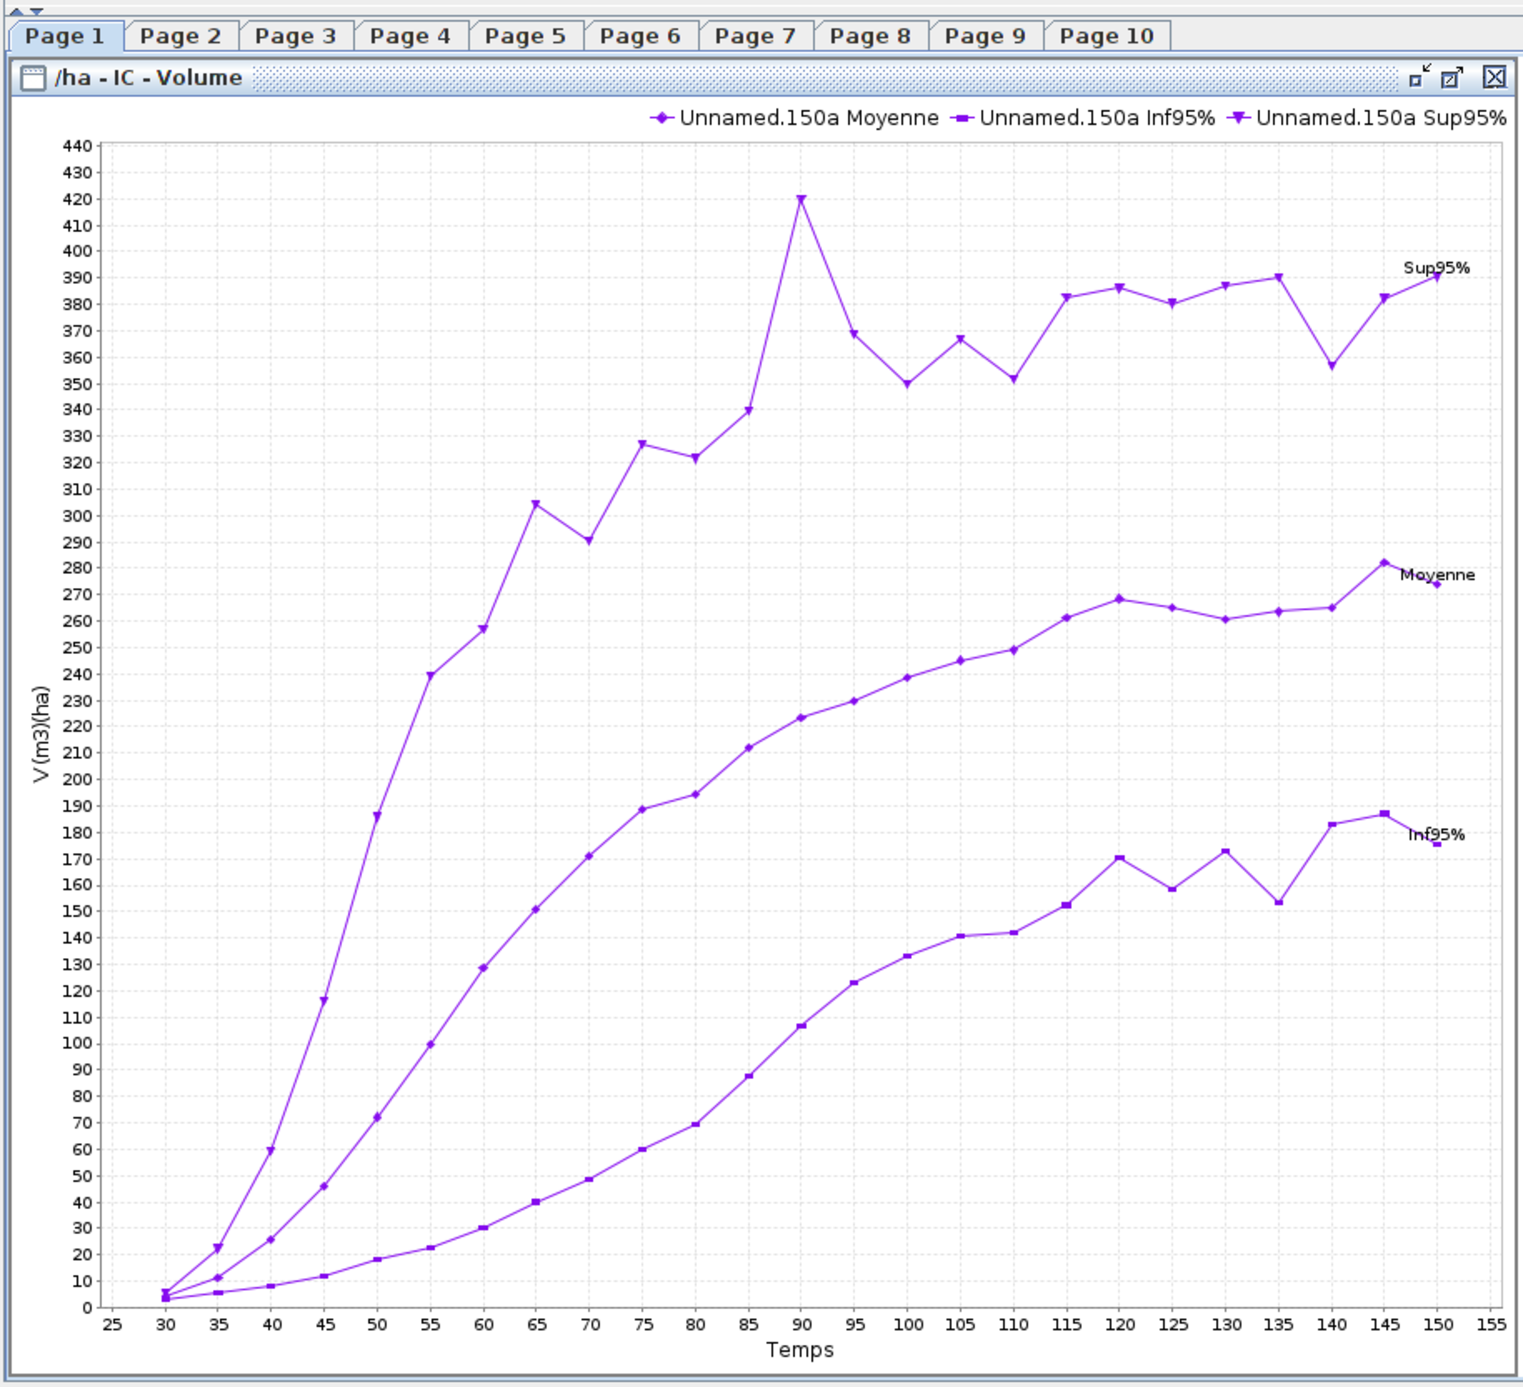
\includegraphics[width=\textwidth]{./figures/evolutionExample3}
\caption{Exemple de simulation stochastique du volume avec un intervalle de confiance de 0.95.}
\label{figureEvolEx3}
\end{center}
\end{figure}

\newpage

\bibliographystyle{apalike}
\bibliography{references}

\newpage

\appendix

\section{Annexe 1 - Espèces considérées}
\label{Annexe1}

Le simulateur MATHILDE considère les espèces typiques de l'association chênaie-hêtraie, soit les espèces principales suivantes:

\begin{itemize}
  \item le chêne sessile (\textit{Quercus petraea})
  \item le chêne pédonculé (\textit{Quercus robur})
  \item le hêtre (\textit{Fagus sylvatica})
  \item le charme (\textit{Carpinus betulus})
\end{itemize}

accompagnées des espèces secondaires telles que

\begin{itemize}
  \item le merisier (\textit{Prunus avium})
  \item le frêne (\textit{Fraxinus excelsior})
  \item l'érable champêtre (\textit{Acer campestre})
  \item les espèces de bouleaux (\textit{Betula} spp.)
  \item les espèces de saules (\textit{Salix} spp.)
  \item le sapin pectiné (\textit{Abies alba})
\end{itemize}

Comme certaines de ces espèces sont trop rares, elles ont été regroupées de la façon suivante: 

\begin{itemize}
  \item les chênes (sessile et pédonculé)
  \item le hêtre
  \item le charme
  \item les autres espèces
\end{itemize}

MATHILDE fonctionne sur la base de ces quatre groupes d'espèces. Lorsque MATHILDE lit un fichier d'inventaire, les codes suivants sont sensés représenter les espèces:

\begin{itemize}
  \item CHS: chêne sessile
  \item CHP: chêne pédonculé
  \item HET: hêtre
  \item CHA: charme
  \item Tout autre chaîne de caractères est assimilée au groupe des autres espèces
\end{itemize}


\end{document}